
\section{Introduction}
The US Department of Defense Integrated Unmanned Systems Roadmap \cite{dod:uavroadmap:2011} defines four levels of autonomy for Unmanned Systems. Level 1 involves manual operator control. Level 2 assumes automatic control while using humans to delegate waypoints. Level 3 assumes the UAV is capable of performing high-level activities using sensed data when given some directions by a human. Level 4 assumes that the UAV is capable of taking a top-level goal, breaking it into tasks and executing them along with the contingency replanning necessary to accomplish a top-level goal. Level 4 approaches the abstract and high-level goals that are provided to human soldiers in today's battlefield.

Level 2 behavior is available in almost all UAV's today. However, this accomplishment is after at least two decades of development with multiple efforts for each type of vehicle. The current U.S Department of Defense focus is on research, development and procurement of technologies that encompass Level 3 and Level 4 autonomous operations while assuming Level 2 is available. The key to developing fully autonomous Level 4 type behaviors is the ability to plan and also deal with contingencies. At the flight control system level this translates to the closed loop system being robust and adaptive to changes in the environment and vehicle dynamics. To motivate further, future Unmanned Systems will involve verification and validation using formal approaches where an amount of trust in autonomy is generated. Current conventional FAA certification practices will be superseded with certification methods that allow integration of UAV's into the civil airspace. One straightforward metric that may be used for 'trust in flight control' is the variance in trajectory tracking with uncertainty in the dynamics and environment. Consequently, the vehicles may be required to perform at their limits in order to maintain the required performance. Most current control systems still do not leverage the full flight envelope of small helicopters, at least, unless significant and expensive system identification and validation has been conducted.

Currently, fast algorithms to plan routes around obstacles are available\cite{Frazzoli.Dahleh.ea:JGCD02,Karaman.Frazzoli:IJRR11}. To be truly useful, these routes would include high-speed dashes, tight turns around buildings, avoiding dynamic obstacles and other required aggressive maneuvers. Allowing control saturation and adaptation allows higher level planning algorithms to provide optimistic trajectories which are then tracked by the flight controller to the best of the vehicles ability. The following is a description of some key elements that affect flight control stability and performance.

\emph{Parametric Uncertainty} arises from uncertainty in the mass, inertia properties, and aerodynamic characteristics. This limits the safe operational envelope of the vehicle to flight regimes where control designs are valid and parametric uncertainty is small. The effects of parametric uncertainty and unmodeled dynamics can be handled using a combination of system identification \cite{gavrilets:gnc:01,civita:ahs:02,mettler} and robust control techniques \cite{civita:gnc:02,gavrilets:gnc:02,civita:acc:03}.  However, system identification is expensive and when changes happen in real-time, for e.g., an unexpected payload is attached or deployed, the available previously-identified models may not fit the current aircraft configuration.  In this chapter, parametric uncertainty arises due to approximate inversion and appears as an unknown nonlinear function of the states and controls (unstructured). An adaptive element (neural network) is then used as a nonlinear function approximator to instantaneously cancel the inversion error.

\emph{Unmodeled Dynamics} arise when the vehicle model used for control design neglects parts of the real system's dynamics. Examples include the Bell-Hillier stabilizer bar and the flapping dynamics of the helicopter rotor blades. For most autonomous flight control work, the flapping dynamics may be safely neglected, whereas the Bell-Hillier stabilizer bar found on small rotorcraft cannot be ignored when high-bandwidth attitude control is desired. This chapter assumes state-feedback of rigid-body states keeping the control design simpler by leveraging the control design's robustness to unmodeled dynamics. Related adaptive designs that use an output-feedback controller formulation to explicitly deal with unmodeled dynamics are described in \cite{calise:automatica:2001} with experimental results in \cite{corban:gnc:2003}.

\emph{Actuator Magnitude and Rate Saturation} limit control authority and thus the closed loop stability and performance. Addressing input dynamics constitutes an important class of control design methods for systems with bounded actuation and include Sontag's universal formula approach using control Lyapunov functions \cite{lin:scl:91} and others \cite{bemporad:itac:97,pappas:cdc:95}. Avoiding saturation, however, usually results in either conservative or highly complex control laws leading to possibly very conservative domains of attraction and slow convergence. See \cite{bernstein:ijrnc:95} and the references therein for a survey of early work on constrained control. 


Other related works on rotorcraft control may be found in \cite{kendoul:itr:2006,kendoul:jgcd:2007,kendoul:jfr:2010} and a recent survey on guidance, navigation and control methods for rotorcraft is available in \cite{kendoul:jfr:2012}.


%A key aspect in the effective use of unmanned aerial vehicles(UAVs) for military and civil applications is their ability to accommodate changing dynamics and payload configurations automatically without having to rely on substantial system identification efforts. Variants of the Neural-Network (NN) based direct adaptive control methods have been used as enabling technologies for practical flight control systems that allow online adaptation to uncertainty. This technology has been successfully applied to the recent U.S. Air Force Reconfigurable Control for Tailless Fighter Aircraft (RESTORE) culminating in a successful flight demonstration \cite{calise:jgcd:01,brinker:jgcd:01} of the adaptive controller on the X-36. A combined inner-outer loop architecture was also applied for guidance and control of the X-33 \cite{johnson:jgcd:03} and evaluated successfully in simulation for various failure cases.

%Much adaptive control work on helicopters has concentrated on improving the tracking performance of attitude commands \cite{nakwan:jgcd:02,leitner:jgcd:97,rysdyk:jgcd:98}.

\begin{figure}
  \centering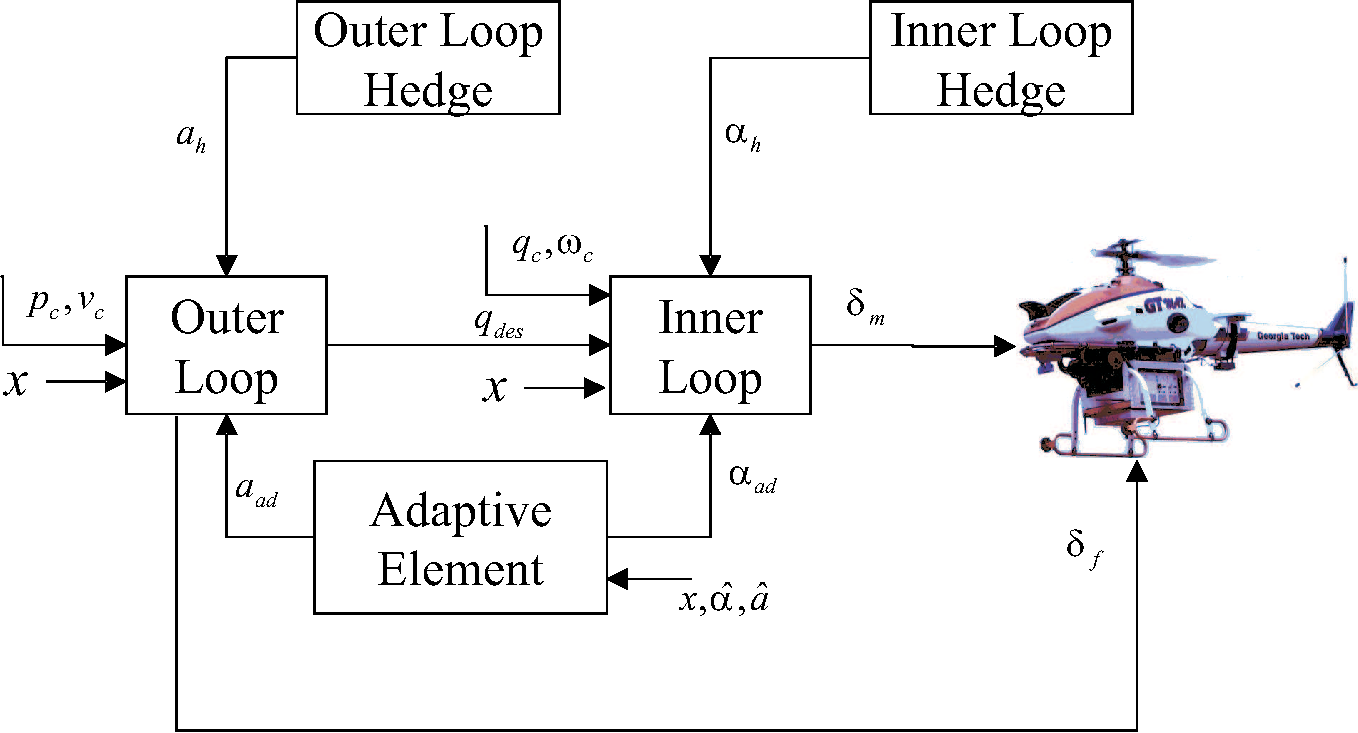
\includegraphics[width=0.7\columnwidth]{overallarch}
  \caption{Overall Architecture}
  \label{f:overallarch}
\end{figure}

\subsubsection*{Approach}
Helicopters have 6 degrees of freedom when considering just the rigid body modes and 4 independent controls are available to control them. Traditionally, the control variables lateral stick, $\delta_{lat}$, longitudinal stick, $\delta_{lon}$ and pedal, $\delta_{ped}$, control moments around the roll, pitch and yaw axes respectively. Finally, the collective input, $\delta_{coll}$ produces thrust along the main rotor shaft. The rotational dynamics are fully actuated whereas the translational dynamics are underactuated, but controllable. The rotor thrust has to be oriented using the aircraft's pitch and roll attitude to produce translational accelerations.

An overall architecture of the approach is shown in \fig{f:overallarch} with details in \fig{f:detailarch}. The outer loop is responsible for tracking desired translational accelerations. It generates $\delta_{coll}$ to vary rotor thrust along the main shaft and also generates the desired roll and pitch angles to orient the thrust vector to generate linear accelerations in these two underactuated degrees of freedom. Note here that the desired pitch and roll angles are commands to the inner-loop controller. In this respect the inner-loop acts like a (virtual) actuator as far as the outer-loop is concerned. Similarly, the inner-loop generates the actuator deflections necessary to control the rotational dynamics. Of course, here the inner-loop's output actuation signal is subject to the real actuator dynamics of the physical aircraft. In both loops, approximate models of the rotational (inner-loop) and translational (outer-loop) dynamics are dynamically inverted to produce the actuator deflections (and desired pitch and roll) necessary to achieve the desired angular and linear accelerations. These desired accelerations are generated using reference models dictating the desired ideal closed loop response. The cascaded inner-outer loop architecture used here is commonly employed in aerospace control applications due to the different dynamical time-scales of the two loops. {\color{red} Chapter ``Linear Flight Control Techniques for Unmanned Aerial Vehicles'' in this book discusses relevant details of cascaded control systems for UAVs.}

Adaptation is introduced in all six degrees of freedom to account for inversion errors arising from the approximate models used for inversion purposes. There is no particular restriction on the inversion that results in \emph{desired} actuator deflections to be bounded. Hence, at large desired accelerations, large actuator deflections may be commanded. Such saturation and dynamics will now appear in the adaptation training signal. This is also true in the case of the outer-loop because the commanded pitch and roll attitudes are now subject to the closed-loop dynamics of the inner-loop in addition to the actuator dynamics of the $\delta_{coll}$ actuator.

These nonlinearities appear in the stability analysis by way of their appearance in the error dynamics.  The, Pseudocontrol Hedging signal (PCH) is introduced in the outer-loop and inner-loop reference models in a manner that exactly removes elements of actuator saturation from the training signal for the adaptive element. The reference models themselves are nonlinear and prescribe the aggressiveness with which external commands are achieved. Thus, a comprehensive nonlinear, adaptive, trajectory tracking controller capable of adapting to uncertainties in all six degrees of freedom is developed. It must be noted that although the concrete example used throughout this chapter is one of a helicopter, the controller is not specific to a helicopter UAS. The development is generic, the only difference between a helicopter, a fixed-wing or other esoteric aircraft is the manner in which the available controls are categorized and the approximate models used for dynamic inversion purposes.

An underlying assumption of this work is that the nonlinear modeling error uncertainty can be approximated by a continuous function over the flight domain of an aircraft. The goal is to capture an approximation of the uncertainty using universal approximators such as neural networks. This universal approximation property guarantees that given a sufficient number neurons, there exists and an optimal set of (a priori unknown) weights that can approximate the uncertainty to a desired minimum approximation error. Once these weights are found, the learned dynamics can be used for online planning and health-monitoring purposes. The baseline adaptive laws developed in later sections of this chapter are designed to cancel instantaneous model error but do not necessarily guarantee convergence to the ideal weights during normal course of operation~\cite{ejohnson:jgcd:2005,kannan:cdc:2010,kannan:phd}. To alleviate this restriction, a modification, the \emph{concurrent learning adaptive control method} is introduced that greatly improves the convergence of weights to their ideal values in real-world conditions~\cite{Chowdhary:JGCD:10}. The method can in fact guarantee exponential convergence of the neural network weights to a neighborhood of their ideal values for linearly parameterized neural networks~\cite{Chowdhary:phd:2010}.

The adaptive controller described in this chapter has been extensively validated in flight on several aircraft regularly since 2002. The range of aircraft types include the Yamaha RMAX (GTMax) helicopter (\fig{f:helipic}), a 11-inch ducted-fan, the GTSpy (\fig{f:gtspypic}), a tail-less fixed-wing aircraft, the D6, and a high thrust-to-weight ratio aircraft, the GTEdge (\fig{f:gtedgepic}). The GTEdge is a tilt-body fixed-wing aircraft and capable of hovering on its propeller and flying like a regular fixed-wing aircraft. An interesting set of maneuvers performed by the GTEdge is the {hover$\Rightarrow$forward-flight$\Rightarrow$hover}, all using the same adaptive control system. The methods discussed here have also been implemented on smaller aircraft such as the GT Twinstar (Figure~\ref{f:twinstarpic}) a foam built twin-engine aircraft, the GT Logo a small rotorcraft of about 1 meter rotor diameter, and the GTQ \cite{chowdhary:gnc11:2011}, a miniature quadrotor. On the GT Twinstar, a variant of the algorithms presented here was used for flight with 25\% right wing missing~\cite{chowdhary:gnc:10:invited,chowdhary:infotech11:2011,Chowdhary:JGCD:12}.
\todo[inline,color=green]{Expand this list of Aircraft}
\todo[inline,color=green]{Need to refer to concurrent learning here}



\begin{figure}
  \centering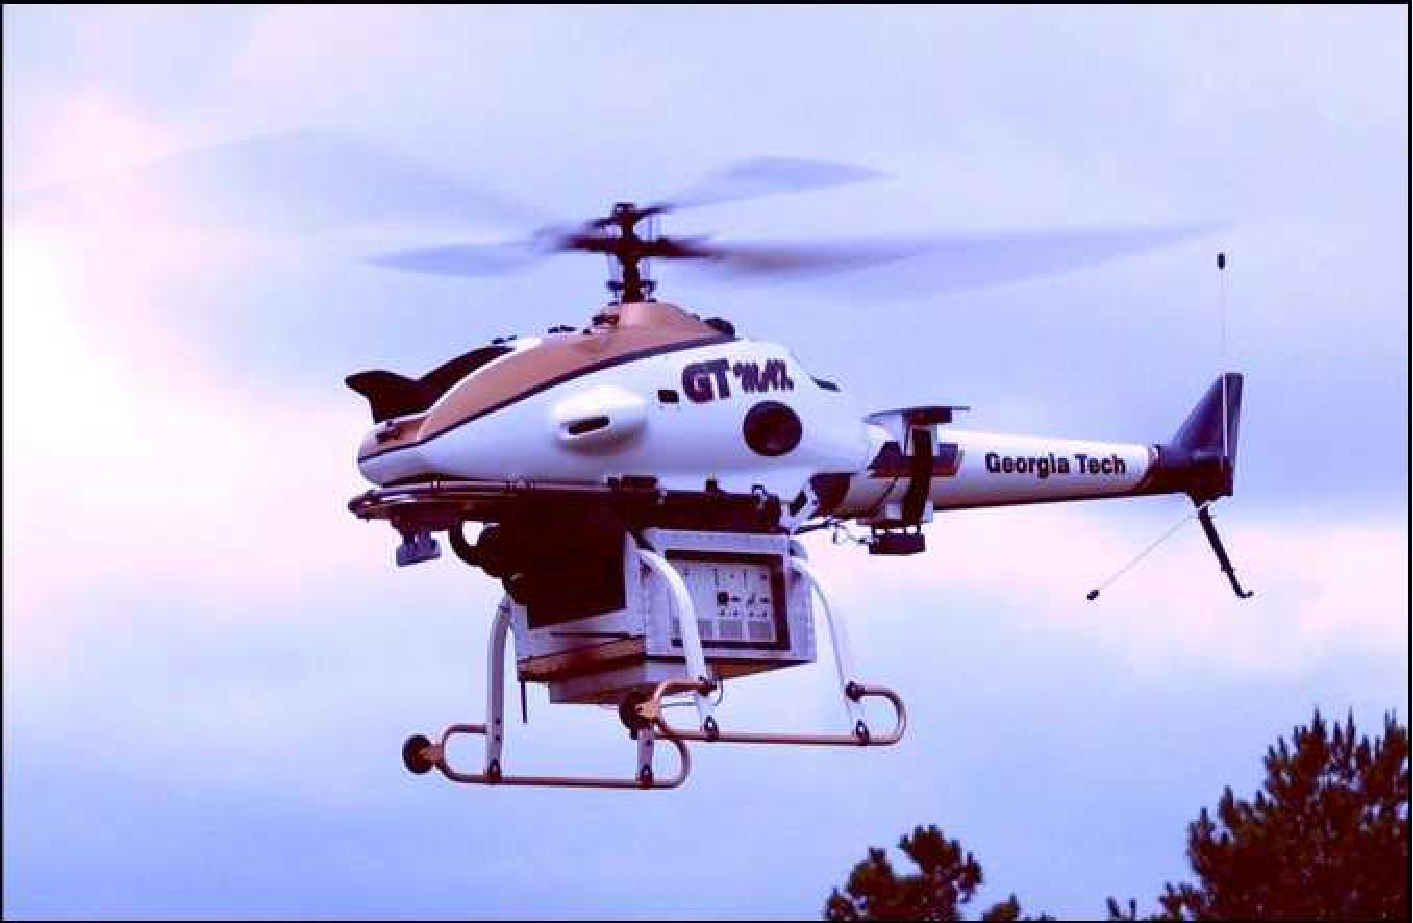
\includegraphics[width=0.7\columnwidth]{helipic}
  \caption{The GTMax Helicopter}
  \label{f:helipic}
\end{figure}
\begin{figure}
  \centering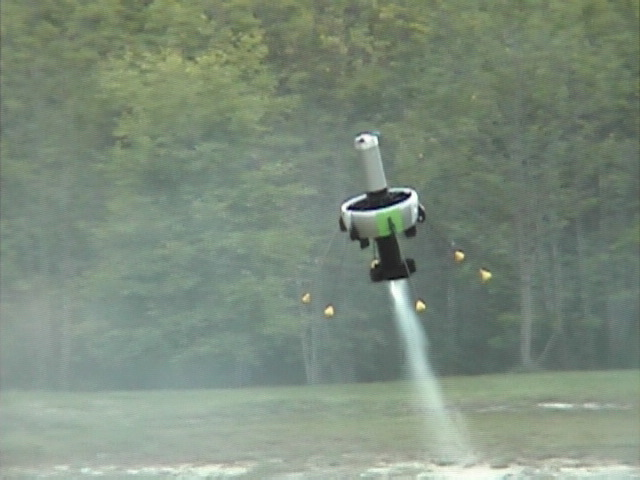
\includegraphics[width=0.7\columnwidth]{gtspy}
  \caption{The GTSpy 11-inch ducted fan}
  \label{f:gtspypic}
\end{figure}

\begin{figure}
  \centering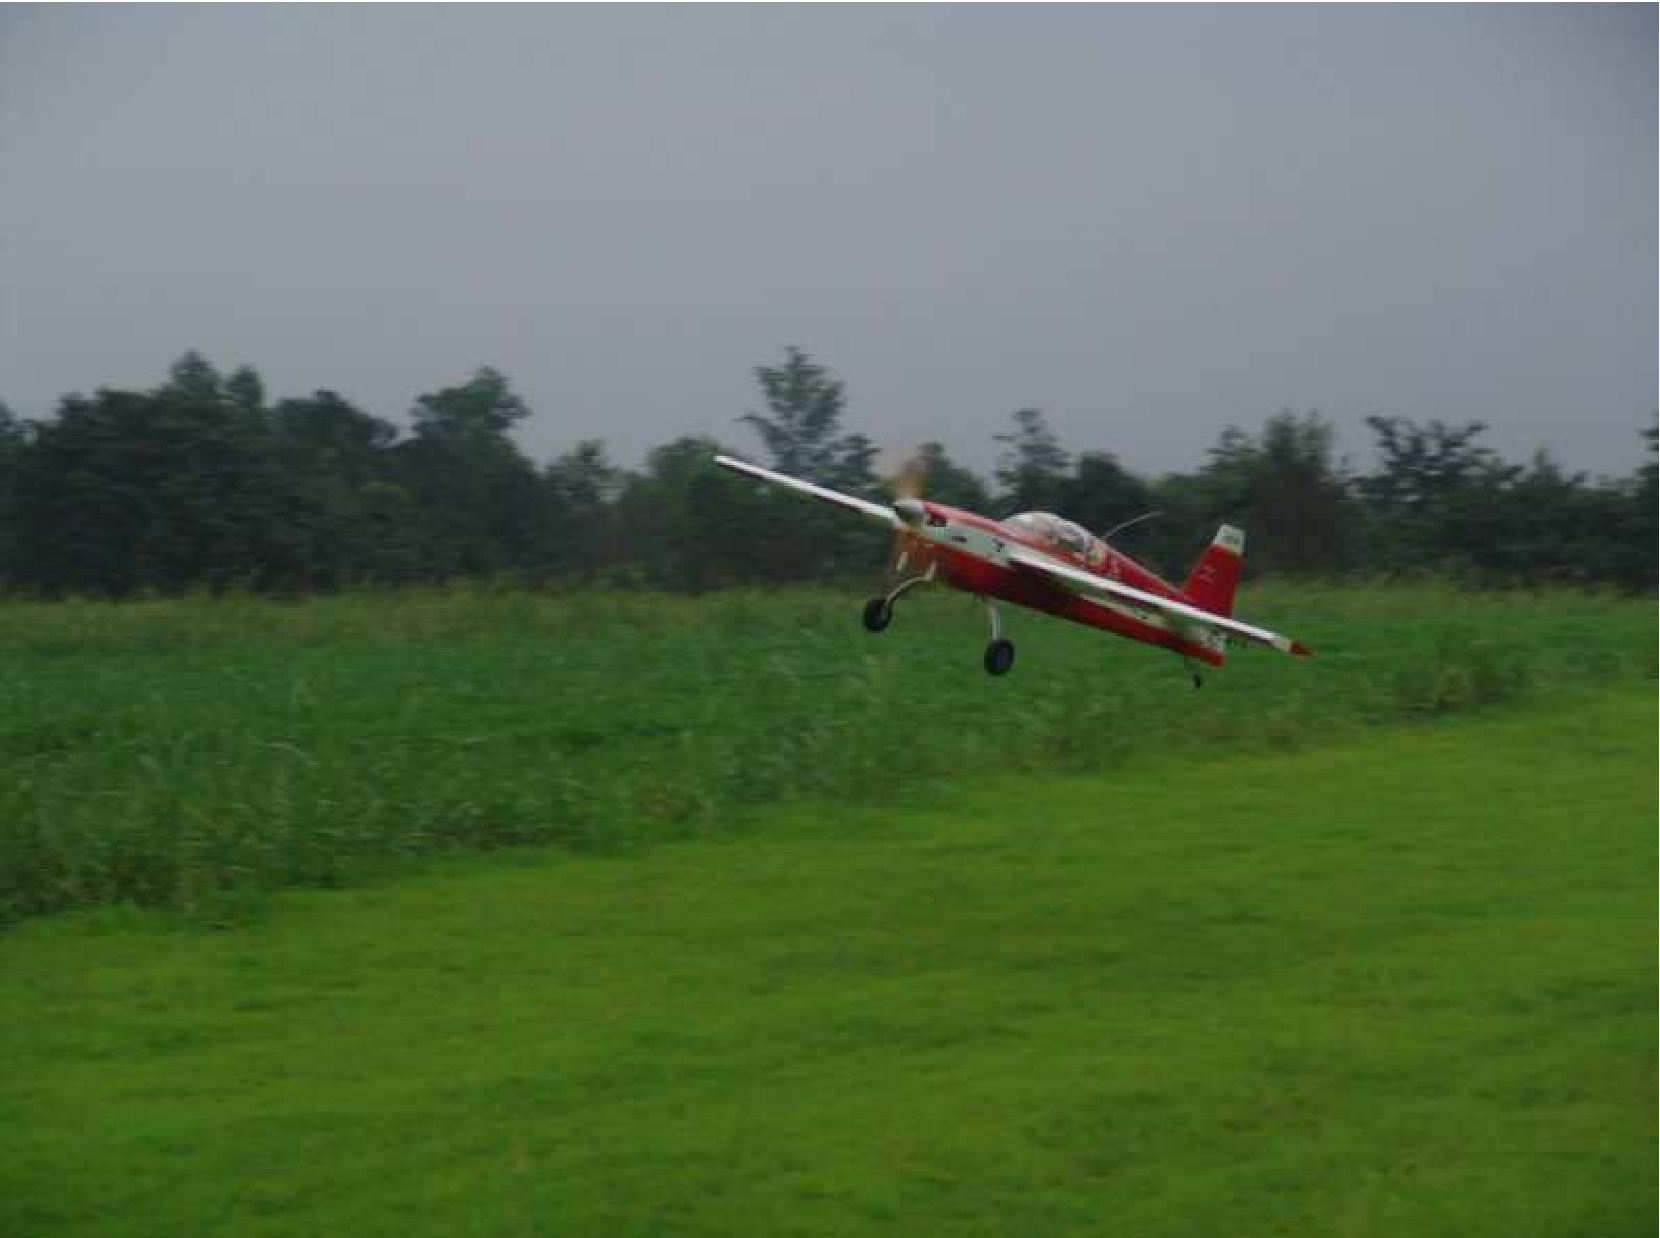
\includegraphics[width=0.7\columnwidth]{gtedge}
  \caption{The GTEdge aircraft with a high (greater than 1) thrust-to-weight ratio}
  \label{f:gtedgepic}
\end{figure}

\begin{figure}
  \centering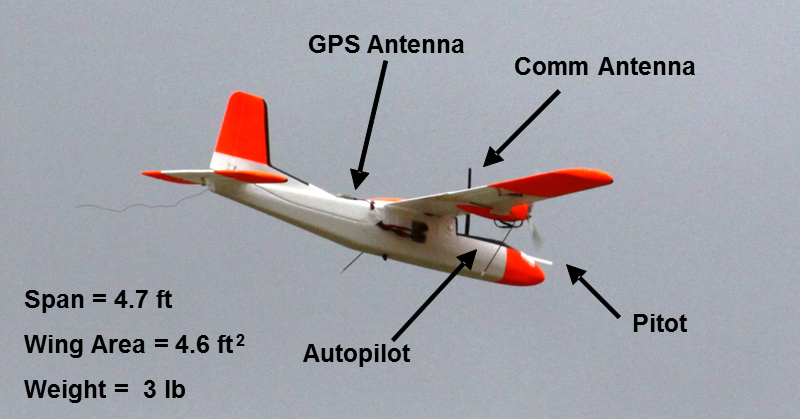
\includegraphics[width=0.7\columnwidth]{twinstar}
  \caption{The GTTwinstar foam built twin engine aircraft equipped for fault-tolerant control work (see e.g. \cite{chowdhary:infotech11:2011})}
  \label{f:twinstarpic}
\end{figure}

